%% ============================================================
% f2012_shandong_arts_q19_pyramid.tex
%% 2012 山东卷（文科）第 19 题 四棱锥 E-ABCD（△ABD 为正三角形，CB=CD）
%% 来源 PDF：普通高考/2012/2012山东文.pdf 第 2 页（印面 762）第 1 栏
%% 坐标取自原页矢量层（bp），原点为图区左上角 (238.0,495.0)，y 向下；虚线照原页。
%% ============================================================
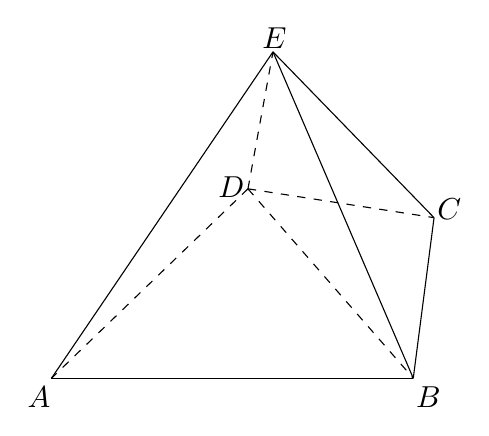
\begin{tikzpicture}[x=1bp,y=-1bp,
  every node/.style={inner sep=0,font=\fontsize{10.5pt}{12.6pt}\selectfont},
  line cap=butt, line join=miter]
  \draw[line width=0.3985bp] (95.695,17.93) -- (153.676,77.609);
  \draw[line width=0.3985bp] (95.695,17.93) -- (15.953,135.418);
  \draw[line width=0.3985bp] (146.195,135.418) -- (153.676,77.609);
  \draw[line width=0.3985bp] (146.195,135.418) -- (15.953,135.418);
  \draw[line width=0.3985bp] (95.695,17.93) -- (146.195,135.418);
  \draw[line width=0.3985bp, dash pattern=on 2.989bp off 2.989bp] (86.684,67.234) -- (95.695,17.93);
  \draw[line width=0.3985bp, dash pattern=on 2.989bp off 2.989bp] (86.684,67.234) -- (153.676,77.609);
  \draw[line width=0.3985bp, dash pattern=on 2.989bp off 2.989bp] (86.684,67.234) -- (15.953,135.418);
  \draw[line width=0.3985bp, dash pattern=on 2.989bp off 2.989bp] (86.684,67.234) -- (146.195,135.418);
  \node[anchor=base west] at (91.64,16.67) {$E$};
  \node[anchor=base west] at (75.87,70.3) {$D$};
  \node[anchor=base west] at (154.63,78.41) {$C$};
  \node[anchor=base west] at (7.18,146.11) {$A$};
  \node[anchor=base west] at (147.02,146.11) {$B$};
\end{tikzpicture}
